% Created 2024-03-08 Fri 16:11
% Intended LaTeX compiler: pdflatex
\documentclass[a4paper, 12pt]{article}
\usepackage[utf8]{inputenc}
\usepackage[T1]{fontenc}
\usepackage{graphicx}
\usepackage{longtable}
\usepackage{wrapfig}
\usepackage{rotating}
\usepackage[normalem]{ulem}
\usepackage{amsmath}
\usepackage{amssymb}
\usepackage{capt-of}
\usepackage{hyperref}
\usepackage[utf8]{inputenc}      % accents
\usepackage[T1]{fontenc}         % PS fonts
\usepackage{newtxtext,newtxmath} % do not use CM fonts
\usepackage{amsmath}             % multi-line and other mathematical statements
\usepackage{setspace}            % setting the spacing between lines
\usepackage{graphicx}            % go far beyond what the graphics package
\usepackage[normalem]{ulem}      % various types of underlining
\usepackage{caption}             % rotating captions, sideways captions, etc.
\usepackage{float}               % tables and figures in the multi-column environment
\usepackage{subcaption}          % for subfigures and the like
\usepackage{longtable}           % tables that continue to the next page
\usepackage{multirow}            % tabular cells spanning multiple rows
\usepackage[table]{xcolor}       % driver-independent color extensions
\usepackage{lipsum}              % loren dummy text
\setlength{\marginparwidth}{2cm} % todonotes' requirements
\usepackage{todonotes}           % todo's
\usepackage{chicago}             % a bibliography style
\usepackage{bookmark}            % Include the bookmark package
\usepackage[a4paper,left=25mm,right=25mm,top=25mm,bottom=25mm,headheight=6mm,footskip=12mm]{geometry}
\setlength{\parindent}{0em}
\setlength{\parskip}{4ex}
\AddToHook{cmd/section/before}{\clearpage}
\usepackage{fancyhdr}
\fancyhf{}                            % clear off all default fancyhdr headers and footers
\rhead{\small{\emph{\projtitle, \projauthor}}}
\rfoot{\small{ \thepage\ }}
\pagestyle{fancy}                     % apply the fancy header style
\renewcommand{\headrulewidth}{0.4pt}
\renewcommand{\footrulewidth}{0.4pt}
\usepackage{color}
\definecolor{engineering}{rgb}{0.549,0.176,0.098}
\definecolor{cloudwhite}{cmyk}{0,0,0,0.025}
\usepackage{listings}
\lstset{language=C, basicstyle=\footnotesize\ttfamily, keywordstyle=\bfseries, numbers=left, numberstyle=\scriptsize\texttt, stepnumber=1, numbersep=8pt, frame=tb, float=htb, aboveskip=8mm, belowskip=4mm, backgroundcolor=\color{cloudwhite}, showspaces=false, showstringspaces=false, showtabs=false, tabsize=2, captionpos=b, breaklines=true, breakatwhitespace=false, escapeinside={\%*}{*)}, morekeywords={*,var,template,new}}
\hypersetup{plainpages=false, pdfpagelayout=SinglePage, bookmarksopen=false, bookmarksnumbered=true, breaklinks=true, linktocpage, colorlinks=true, linkcolor=engineering, urlcolor=engineering, filecolor=engineering, citecolor=engineering, allcolors=engineering}
\graphicspath{{figures/}}
\newcommand{\school}{Universidad Carlos III de Madrid}
\newcommand{\degree}{Dual Bachelor in Data Science and Engineering and Telecommunication Technologies Engineering}
\newcommand{\projtitle}{Laboratory Report}
\newcommand{\subtitle}{Integrated Circuits and Microelectronics}
\newcommand{\projauthor}{Andrés Navarro Pedregal (100451730) \& Daniel Toribio Bruna (100454242)}
\newcommand{\tutor}{}
\newcommand{\windspt}{\textsf{WindsPT\/}}
\newcommand{\windscannerpt}{\emph{Windscanner.PT\/}}
\newcommand{\class}[1]{{\normalfont\slshape #1\/}}
\newcommand{\svg}{\class{SVG}}
\newenvironment{info}[1]{\vspace*{6mm}\color{blue}[ \textbf{INFO:} \begin{em} #1} {\vspace*{3mm}\end{em} ]}
\newenvironment{infoopt}[1]{\vspace*{6mm}\color{blue}[ \textbf{INFO (elemento opcional):} \begin{em} #1} {\vspace*{3mm}\end{em} ]}
\author{Andrés Navarro Pedregal and Daniel Toribio Bruna}
\date{\today}
\title{Laboratory Report}
\hypersetup{
 pdfauthor={Andrés Navarro Pedregal and Daniel Toribio Bruna},
 pdftitle={Laboratory Report},
 pdfkeywords={},
 pdfsubject={},
 pdfcreator={Emacs 29.2 (Org mode 9.7)}, 
 pdflang={English}}
\begin{document}

\begin{titlepage}
\center

\vspace{-15mm}
{\large \textbf{\textsc{\school}}}\\

\vfill

{\Large \textbf{\projtitle}}\\[8mm]
{\large \textbf{\subtitle}}\\[28mm]

{\Large \textbf{\projauthor}}\\

\vfill


\includegraphics[width=52mm]{./img/uc3m_logo.png}

\vfill

{\large \degree}\\[8mm]

%\renewcommand{\today}{15 de dezembro de 2023}
\today

\end{titlepage}
\tableofcontents
\section{Introduction}
\label{sec:orgfb58a17}
In this lab report, our goal is to create a waveform generation and FIR (Finite Impulse Response) filter implementation. Our objective is to understand and construct circuits that can generate sinusoidal signals and filter them effectively. These circuits will be designed to operate on FPGA (Field-Programmable Gate Array) boards, specifically the Basys 3 model, utilizing components such as LEDs and digital-to-analog converters (DACs).

Session 1: Waveform Generator
In our first session, we create a circuit capable of generating sinusoidal signals represented with 8 bits of precision. This circuit will be responsible for producing these signals at different frequencies, which will be selected through input switches. The generated waveform will be visualized through both LEDs on the FPGA board and an 8-bit DAC (Pmod R2R), ensuring versatility in signal output. Our design will consist of various components including timers, memory units, and counters to facilitate accurate signal generation and display.

Session 2 and 3: FIR Filter Implementation
Moving forward, we implement a digital FIR filter alongside the previously developed waveform generator. The FIR filter serves the purpose of refining the generated signals by attenuating frequencies beyond a specified cutoff point. Utilizing filter coefficients obtained from MATLAB, we construct a filter with a predetermined number of stages to achieve the desired filtering effect. Integrating this filter into our existing circuitry, we aim to enhance the quality of the generated signals for various applications.

Throughout these sessions, we'll engage in simulation, synthesis, and practical implementation of our designs on FPGA boards. Additionally, we'll document our progress through test benches, oscilloscope measurements, and final reports, ensuring a comprehensive understanding of the design process and its outcomes.

By the end of these sessions, we anticipate gaining valuable insights into circuit design, signal processing, and FPGA-based system implementation, laying a solid foundation for further exploration in the field of integrated circuits and microelectronics.
\section{Design Characteristics}
\label{sec:org5b89b9e}

\subsection{Full Implemented Functionality}
\label{sec:org15b74cb}
\subsection{I/O Interface, Type And Functionality}
\label{sec:orgead3300}
\section{Design Structure}
\label{sec:org0f2b84f}

\subsection{Block Diagram}
\label{sec:org7e9f4b0}

\subsection{Component Description}
\label{sec:orgdbe5901}

\subsection{Calculation}
\label{sec:org08c0ae7}

\subsubsection{Frequencies}
\label{sec:org4895a3e}
\begin{enumerate}
\item Values:
\label{sec:org4c511d0}

We calculated 16 values of a sine signal with the following code:

\begin{verbatim}
import math

 # Define parameters
amplitude = 127
frequency = 1  # Adjust frequency as needed
num_points = 16

 # Generate values
values = []
for t in range(num_points):
        values.append((int) (amplitude * math.sin((2 * math.pi * t) / num_points)))

 # Print the values
for i, val in enumerate(values):
        print(f"f(t_{i}) =", val)
\end{verbatim}

\begin{verbatim}
f(t_0) = 0
f(t_1) = 48
f(t_2) = 89
f(t_3) = 117
f(t_4) = 127
f(t_5) = 117
f(t_6) = 89
f(t_7) = 48
f(t_8) = 0
f(t_9) = -48
f(t_10) = -89
f(t_11) = -117
f(t_12) = -127
f(t_13) = -117
f(t_14) = -89
f(t_15) = -48
\end{verbatim}
\item Periods:
\label{sec:orge9e8149}

The frequencies we needed to use were 600, 1000, 2200, and 3900 Hz. For the period, we calculated that with the following code

\begin{verbatim}
frequencies = [600, 1000, 2200, 3900]
num_points = 16
clock_frequency = 10e7

 # Generate values
values = []
for i in range(len(frequencies)):
        values.append((int) (clock_frequency / (frequencies[i] * num_points)))

 # Print the values
for i, val in enumerate(values):
        print(f"time({i}) =", val)
\end{verbatim}

\begin{verbatim}
time(0) = 10416
time(1) = 6250
time(2) = 2840
time(3) = 1602
\end{verbatim}
\end{enumerate}
\subsubsection{Filter Coefficients}
\label{sec:org913ebc1}

For the coefficients of the filter, we used a 12 order filter, therefore we needed 13 different values. The calculations can be seen below.

\begin{center}
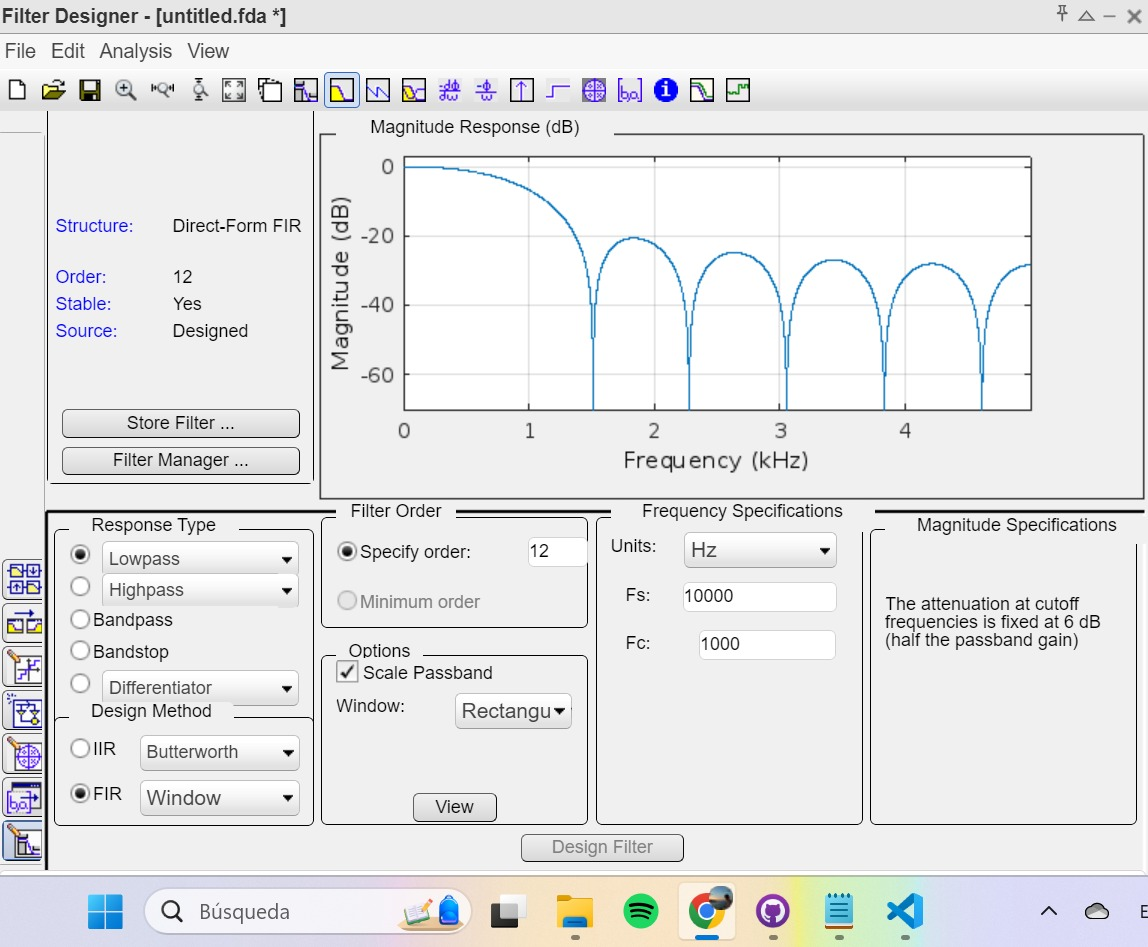
\includegraphics[width=.9\linewidth]{./img/filter_coefficient_matlab.jpg}
\end{center}

\begin{center}
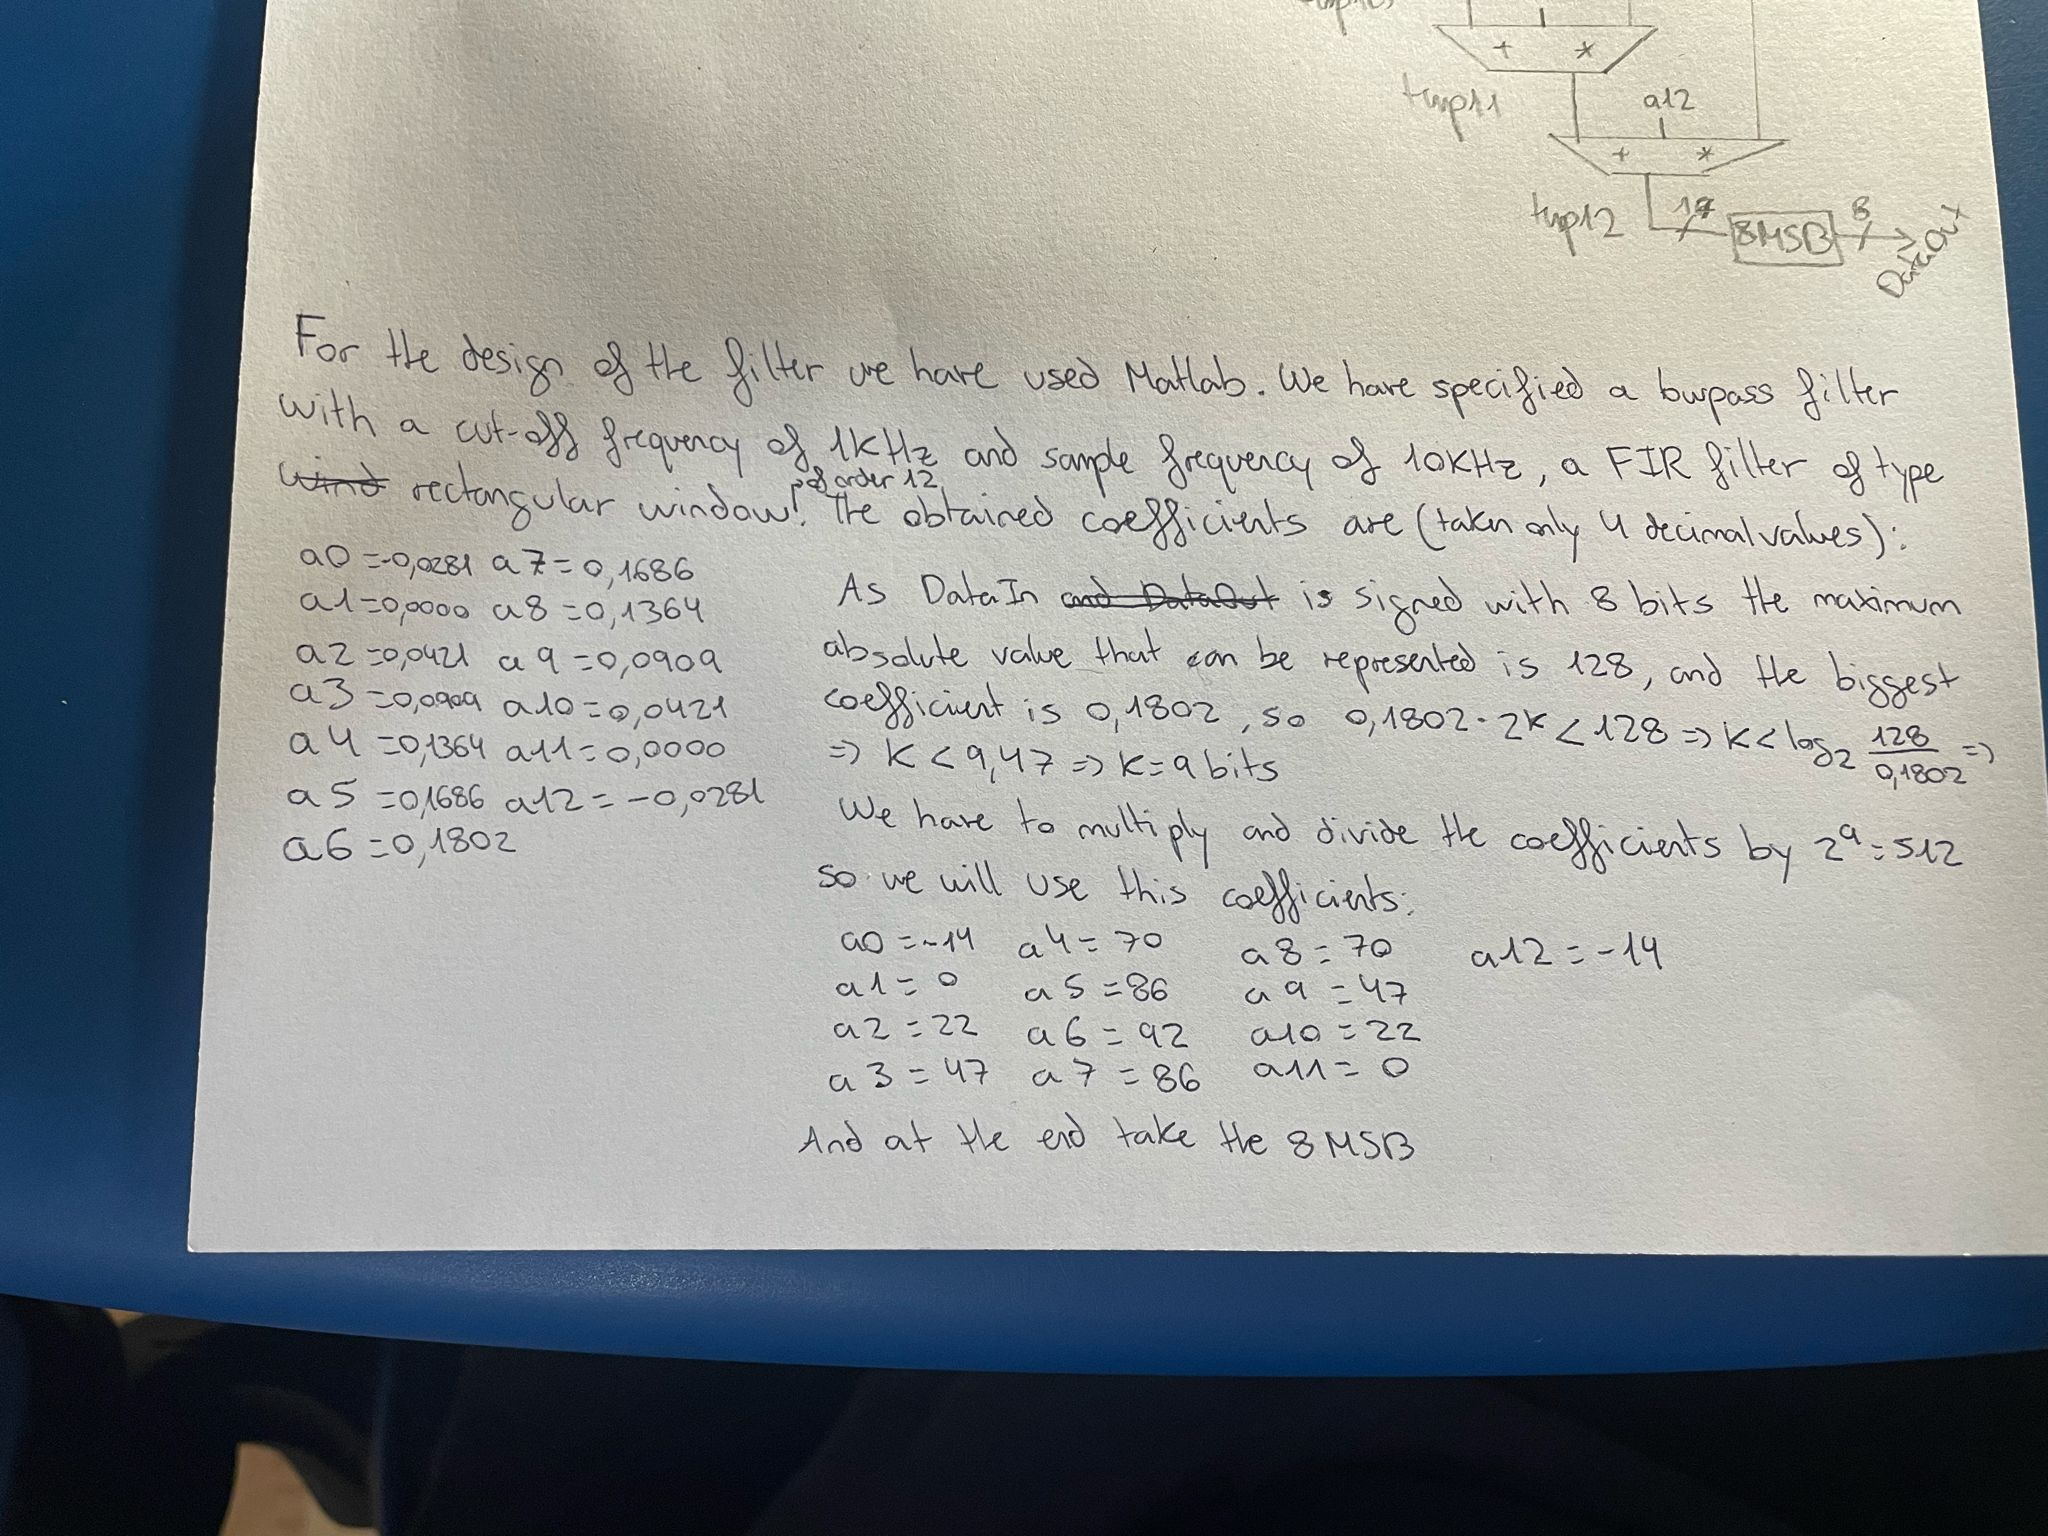
\includegraphics[width=.9\linewidth]{./img/filter_coefficient_calculations.jpg}
\end{center}
\subsection{Simulations}
\label{sec:org76c61fd}

For the simulations, 2 periods of each signal where performed. Note that the filter has a cutoff frequency of 1000 Hz.

For the first frequency, the signal passes without a problem. For the second frequency, it reduces by half as it is the same as the cutoff frequency where the filter will attenuate the signal by one half. And for the other signals, the filter filters out completelly the sine wave.

\begin{center}
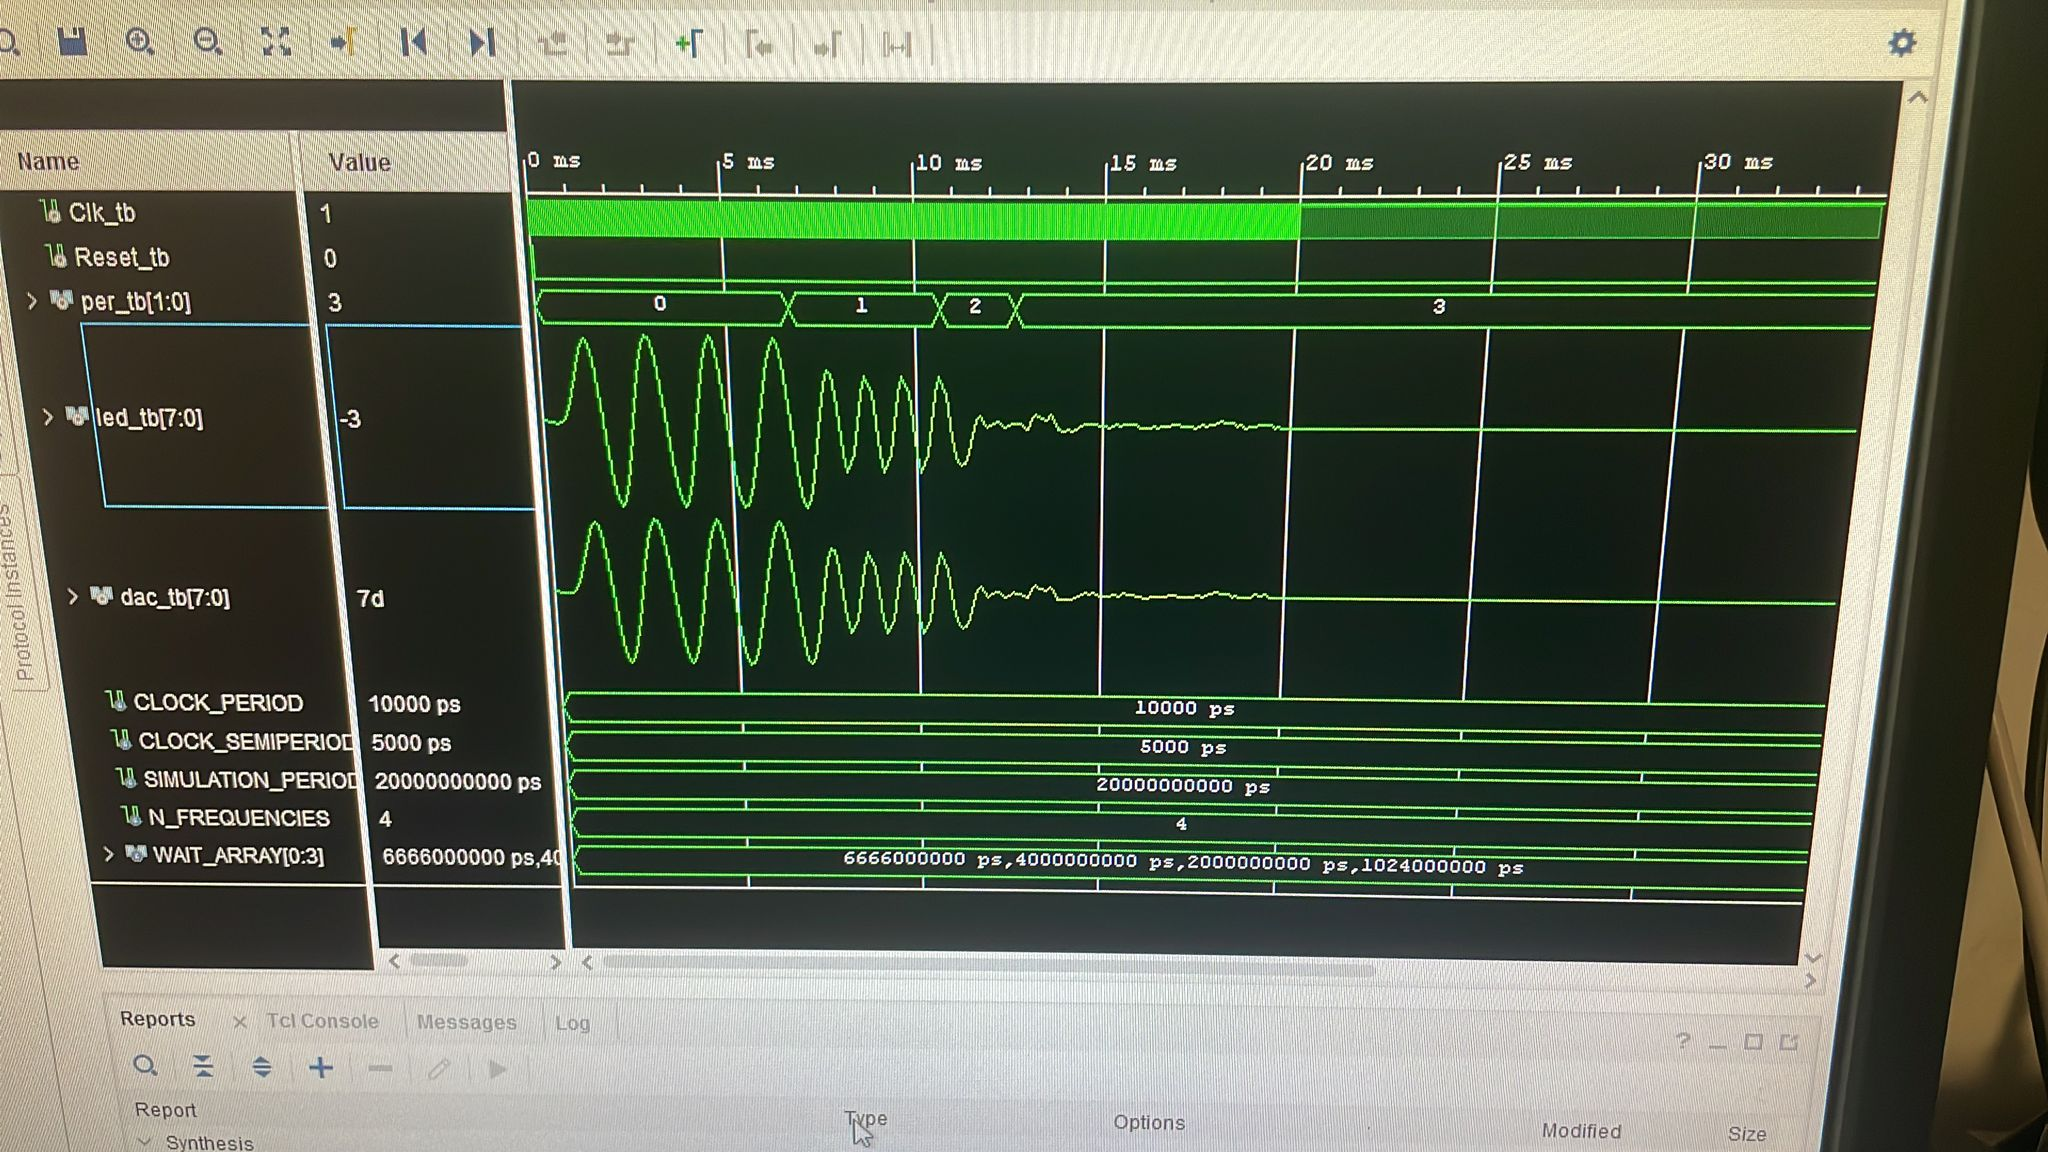
\includegraphics[width=.9\linewidth]{./img/simulation.jpg}
\end{center}
\section{Architectures}
\label{sec:org6336008}

Different architectures have been proposed to reduce the critical region of the filter so we can use higher frequencies. Note, that the VHDL code is separated in different files for each filter.
\subsection{Parallel Architecture}
\label{sec:org03e821b}

For the parallel architecture, we use the following diagram.

This architecture has a big critical region compared to the pipeline architecture as there are no intermediate registers to save the information.
\subsection{One Flip-Flop Pipeline Architecture}
\label{sec:org19951ec}

For the pipeline architecture with one intermediate step, we use the following diagram.

We added a single temporary flip-flop to reduce the critical region of the filter by half. Therefore, we expect that even though we will increase the area of the implementation we increase the maximum frequency that the filter can work at.
\subsection{Two Flip-Flop Pipeline Architecture}
\label{sec:orgd61567e}

For the final part, we added a second stage in the pipeline architecture to see if it further increases the maxiumum frequency.
\section{Synthesis Results}
\label{sec:org6b9474c}

\begin{center}
\begin{tabular}{lrrr}
 & Parallel & One Flip-Flop Pipeline & Two Flip-Flop Pipeline\\
\hline
Logic LUTS & 462 & 465 & 462\\
Flip Flop Registers & 136 & 161 & 186\\
WPWS &  &  & \\
Max Frequency &  &  & \\
\end{tabular}
\end{center}

As we can see in the results from the table above our assumptions are correct. As the pipeline architecture is an implementation of the parallel one but with more registers to save temporary data, the number of flip-flops, therefore the area increases the more intermediate steps we add.

This temporary registers are used to reduce the critical region of the filter so the filter can be used at higher frequencies as seen.

Finally, the LUTS (look up tables) stay almost constant among the 3 architectures analyzed. This is as the computations are the same for the 3 cases.
\section{Conclusion}
\label{sec:org165bd0a}
\end{document}
